\chapter{Implementação dos Algoritmos}
Para implementar as rotinas descritas na seção anterior, optou-se pela linguagem python, com características de maior flexibilidade e menor verbosidade. Na própria linguagem foi implementado também algumas funções para auxiliarem na geração dos elementos nos formatos requisitados, no arquivo \textit{gerar\_entradas.py}. 

A função para criação de listas para entrada recebe como parâmetro, além do número de elementos a ordenação. O parâmetro "ASC" gera elementos ordenados crescentemente, "DESC" decrescentemente e na ausência do parâmetro, os elementos são gerados aleatoriamente. No script de execução, os mesmos elementos gerados são passados para execução e medição pelos 3 algoritmos, de forma que o arquivo de entrada é salvo para conferência apenas.

\begin{figure}[!htb]
\centering
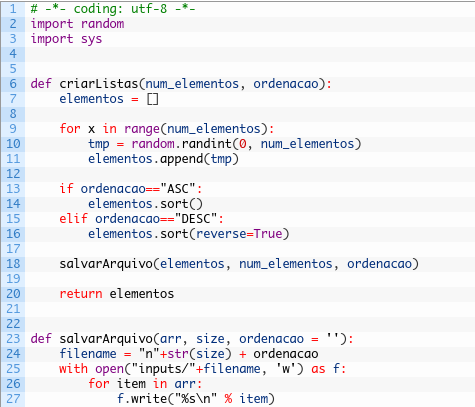
\includegraphics[width=9cm]{img/codigo1.png}
\caption{Funções para geração dos elementos e armazenamento em arquivo}
\label{fig:codigo1}
\end{figure}

No arquivo \textit{sort.py}, a função principal recebe dois parâmetros da linha de comando: o número de elementos a serem testados e a ordem (que segue os mesmos critérios descritos na geração). Para exemplificar, para fazer uma execução para 10 mil elementos ordenados crescentemente, a execução seria: \textit{python sort.py 10000 ASC}. A mesma entrada é processada pelos 3 algoritmos, que têm seu tempo de execução e número de operações individualmente calculados. Os dados são entregues ao arquivo de saída com nome padronizado. Os dados da execução do Tim Sort, por exemplo, são adicionados ao arquivo \textit{tim n10000ASC}.


\begin{figure}[!htb]
\centering
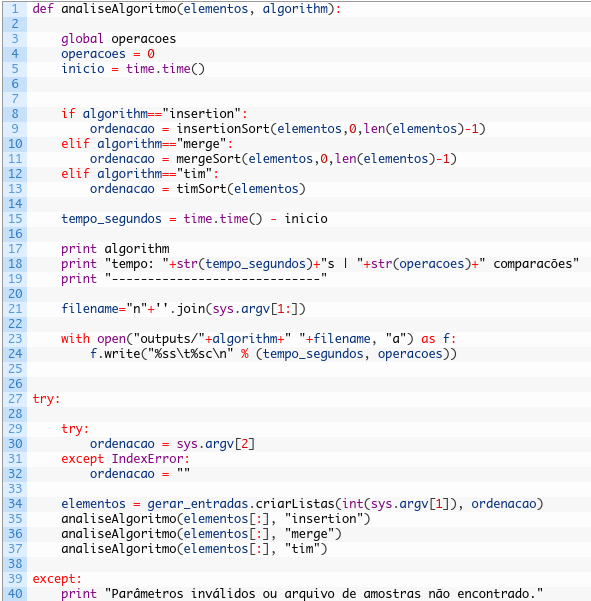
\includegraphics[width=12cm]{img/codigo1-2.png}
\caption{Função principal para execução e análise dos algoritmos}
\label{fig:codigo1-2}
\end{figure}


O primeiro algoritmo a ser implementado foi o Insertion Sort, de funcionamento mais intuitivo e que requer poucas linhas de código. A função recebe, além do vetor de elementos a ser ordenado, um índice de início e outro de fim, que serão utilizados posteriormente nas sub-ordenações do Tim Sort. Em uma execução comum, esses índices são 0, e tamanho do vetor - 1, respectivamente. O laço mais externo percorre o vetor apontando o elemento corrente a ser posicionado, enquanto o laço mais interno vai retornando pela sub-lista ordenada, até identificar o posicionamento do elemento, de forma que a sub-lista se mantenha ordenada.

\begin{figure}[!htb]
\centering
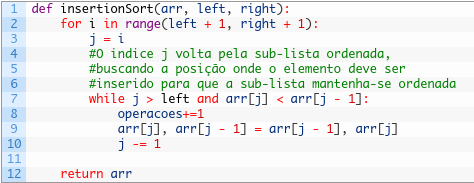
\includegraphics[width=12cm]{img/codigo2.png}
\caption{Função com a implementação do Insertion Sort}
\label{fig:codigo2}
\end{figure}

A implementação do Merge Sort é subdividida em 2 funções. A função principal, \textit{mergeSort}, é responsável por subdividir recursivamente o vetor até que se obtenha um elemento único, que por definição já está ordenado. A função merge, faz o processo de volta, onde os elementos são mesclados em sub-listas ordenadas. 

O processo de ordenação em si se dá na iteração em que o índice \textit{i} itera sobre a lista da esquerda e \textit{j} itera sobre a lista da direita. Partindo do princípio de que cada sub-lista, partindo do elemento único, está ordenada, os índices iteram de forma que se posicionam no menor elemento corrente de cada sub-lista, de forma a compará-los e remover sempre o menor elemento entre eles, mantendo a lista mesclada em ordem.


\begin{figure}[!htb]
\centering
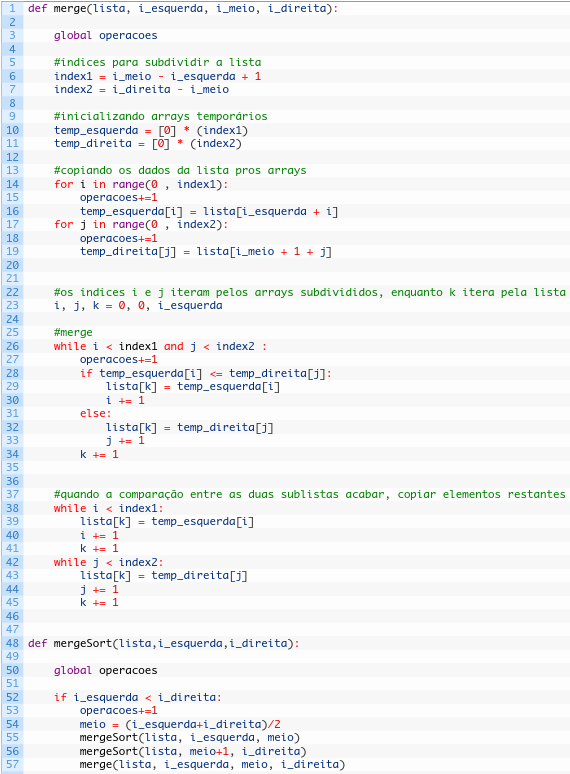
\includegraphics[width=16cm]{img/codigo3.png}
\caption{Funções implementadas para o Merge Sort}
\label{fig:codigo3}
\end{figure}

O Tim Sort, por sua vez, combina os algoritmos implementados anteriormente em uma estratégia que utiliza a vantagem do Insertion Sort para elementos que eventualmente estejam ordenados em sub-conjuntos do vetor principal, sem cair no seu pior caso. O vetor principal é dividido nos subconjuntos denominados \textit{runs}, que serão ordenados pelo Insertion Sort. 

O tamanho desses subconjuntos, segundo princípios e análises do autor, performam bem variando entre 32 a 65 elementos. Para tirar vantagem do fato de que o Merge Sort funciona melhor com conjuntos que têm aproximadamente o mesmo tamanho e sejam base de 2, o tamanho foi eleito em 32 elementos. Após ter os sub-conjuntos ordenados pelo Insertion Sort, o Tim Sort mescla os elementos dessas sub-listas utilizando a função \textit{merge} previamente implementada, até obter a lista original completamente ordenada.

\begin{figure}[!htb]
\centering
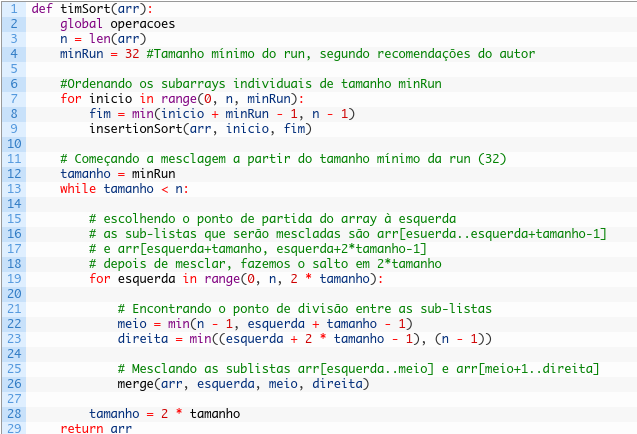
\includegraphics[width=15cm]{img/codigo4.png}
\caption{Implementação do Tim Sort}
\label{fig:codigo4}
\end{figure}
